\subsection{Harmonizome: curated versus systematic annotation density}
\label{sec:harmonizome}
Several earlier audits found the gated panel better studied than background
in curated resources (IntAct degree, HPA immunofluorescence coverage) while
systematic measurement (BioPlex) removed the degree gap. We tested whether
this pattern holds in one independent integrator. Harmonizome (Ma'ayan Lab)
turns about 170 omics, curated and text-mined datasets into thresholded
gene--attribute associations. We fetched the full association profile of
each study gene (203 of 205 resolved) and split datasets by a name
rule fixed before any group comparison: 78 curated/literature datasets,
97 systematic datasets, 2 unclassified and excluded.

\paragraph{Calibration gate.} Pre-registered gates PASSED: (G1) 203
genes resolved (threshold 180); (G2) the CD19 sentinel carries 11{,}116
associations (threshold 1{,}000); (G3) all four housekeeping controls carry at
least 1{,}000 associations (minimum observed 8{,}825).

\paragraph{Hypothesis H1 (falsified).} H1 predicted that gated genes exceed
background in curated associations (one-sided test) but not in systematic
ones (two-sided $p\ge 0.05$). Curated medians were 2510.5 versus 1060
(Mann--Whitney $p=6.3\times10^{-10}$), but systematic medians were also higher,
6548.5 versus 3735 ($p=1.9\times10^{-10}$). The curated share of each gene's
associations was higher in gated genes as well (0.29 versus 0.20,
$p=0.0011$). H1 is falsified: the gap is not limited to curated resources.

\paragraph{Control H2 (falsified, effect shrinks).} After H1 failed we
declared one explanation before testing it: systematic Harmonizome
associations are mostly thresholded expression scores, and gated genes
were chosen for tumour-restricted, high-variance expression, so they collect
more extreme calls.
H2 predicted no gap once systematic data are limited to the 37
non-expression datasets (copy number, mutation, dependency, transcription
factor binding, predicted targets, kinase and localisation maps).
Expression datasets carry the largest gap (medians 5260.5 versus 2571,
$p=2.5\times10^{-12}$). In non-expression datasets the gap shrinks to 1177 versus
930 but stays significant ($p=0.017$), so H2 is also falsified.
The gated panel is more densely annotated than background on every Harmonizome axis, curated and systematic alike. Expression data carry most of the excess (median ratio 2.05 versus 1.27 for non-expression data), which fits selection for tumour-restricted expression, but a smaller residual gap remains. The earlier curated-only reading of the study-bias pattern does not generalise to this integrator.

\paragraph{AND-gate antigens.} CA9 9429 associations (curated share 0.41); CA12 15580 associations (curated share 0.12); CLDN18 4424 associations (curated share 0.27); CLDN6 4298 associations (curated share 0.25); MSLN 9439 associations (curated share 0.24); PSCA 7742 associations (curated share 0.20); SLC39A6 9342 associations (curated share 0.12).

\begin{figure}[t]
\centering
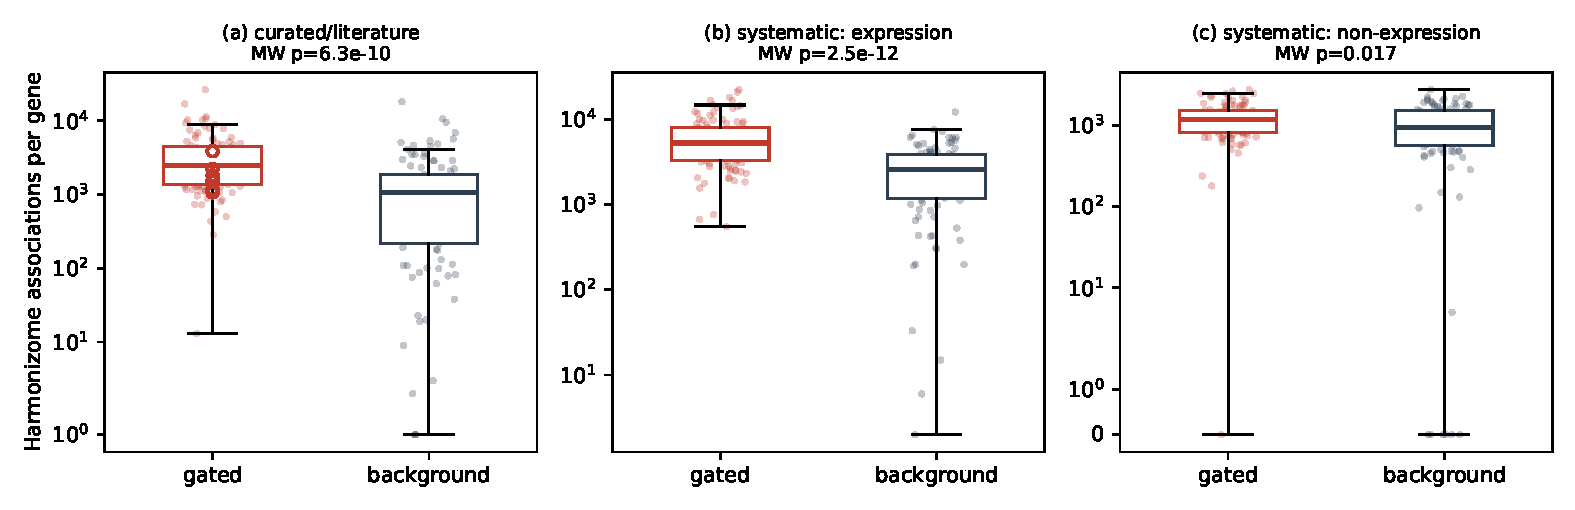
\includegraphics[width=\linewidth]{harmonizome_fig.pdf}
\caption{Harmonizome associations per gene (symlog axis), gated versus
background, in (a) curated/literature, (b) systematic expression and (c)
systematic non-expression datasets. AND-gate antigens are ringed in (a).}
\label{fig:harmonizome}
\end{figure}
